\chapter{Introduction}
\section{Parallel sparse matrix-vector multiplication}
Matrices are one of the most important mathematical objects, as they can be used to represent a wide variety of data in many scientific disciplines: they can encode the structure of a graph, define Markov chains with finitely many states, or possibly represent linear combinations of quantum states or also the behaviour of electronic components. 

In most real-world computations, the systems considered are usually of very large size and involve \textbf{sparse} matrices, because the variables at hand are usually connected to a limited number of others (for example, a very large graph in which each node has just a handful of incident edges); therefore, the matrices involved have the vast majority of entries equal to 0.

More formally, let us consider a matrix of size $m \times n$ with $N$ nonzeros. We say that the matrix is sparse if $ N \ll mn $.

One of the most fundamental operations performed in these real-world computations is the sparse matrix-vector multiplication: in which we compute

\begin{align}
	u:=Av,
	\label{uAv}
\end{align}

where $A$ denotes our $m \times n$ sparse matrix, $v$ denotes a $n \times 1$ dense vector, and $u$ the resulting $m \times 1$ vector.

The computation of this quantity following the definition of matrix-vector multiplication, i.e. with the sum 

\[ 
	u_i = \sum_{j=0}^{n-1} a_{ij} v_j, \quad \text{for }\; 0 \leq i < m,
\]

requires $\mathcal{O}(n^2) = \mathcal{O}(mn)$ operations; this is not very efficient if we have a sparse matrix: if we perform the multiplications only on the nonzero elements, we obtain an algorithm with running time $\mathcal{O}(N)$, and by definition of sparsity we have that $N \ll mn$.

As mentioned, the systems considered are very large, with sparse matrices with thousands (even millions) of rows and columns and millions of nonzeros; for such big instances, even a running time of $\mathcal{O}(N)$ might be non-negligible, especially since sparse matrix-vector multiplications are usually just a part of a bigger iterative algorithm, and need to be performed several times.

It is a very important goal then to be able to perform such computations in the least amount of time possible: however, as there is a natural tradeoff between power consumption and the speed of the processing units \cite{rabaey1996digital}, it is not feasible to rely only on very fast CPUs, but rather focus on parallelism and employ a large number of them with lower processing speed (and, as a result, with fairly low energy requirements).

To describe an efficient way of performing parallel sparse matrix-vector multiplications, we follow the approach described in \cite{BSP}: before the actual computation takes place, the sparse matrix is distributed among the $p$ processors, creating a \textbf{partitioning} of the set of the nonzeros: $A$ is split into $A_0,\dots,A_{p-1}$ disjoint subsets. Moreover, also the input vector $v$ and the output vector $u$ are distributed among the $p$ processors (note that their distribution might not necessarily, and usually it is not, the same).

Figure \ref{fig:partition} shows an example of such distribution, in which a $5 \times 5$ matrix $A$ with 13 nonzeros and the two vectors $u$ and $v$ are split up among two processors, 0 and 1 (denoted, respectively, by the gray and the black color).

\begin{figure}[h]
	\centering
	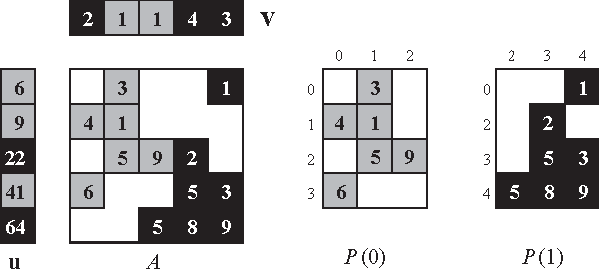
\includegraphics{img/partition}
	\caption{Example of a possible distribution among 2 processors of a 5x5 matrix, and the input and output vectors, as taken from \cite[Fig. 4.3]{BSP}.}
	\label{fig:partition}
\end{figure}

After this distribution, every processor has to compute its local contribution toward the matrix-vector multiplication: to do so, it requires the appropriate vector components which might have been assigned to another processor during the data distribution; if this is the case, communication is required. 

Once all the required vector components are obtained, the processor starts computing all its local contributions, which are afterwards sent to their appropriate owner, according to the distribution of $u$.

The three phases that describe this process for processor $s=0,\dots,p-1$, are summarized in Algorithm \ref{alg:matvec}, from \cite{BSP,mondriaan}.  

\begin{algorithm}[h]
	\begin{algorithmic}
		\Require{$A_s$, the local part of the vector $v$}
		\Ensure{The local part of the vector $u$}
		\State
		\State 	$I_s := \left\{ i | a_{ij} \in A_s \right\}$
		\State 	$J_s := \left\{ j | a_{ij} \in A_s \right\}$
		\State
	\end{algorithmic}
	\begin{enumerate}[(1)]
			\setcounter{enumi}{-1}
		\item 	\begin{algorithmic} \Comment{Fan-out}
				\ForAll{$j \in J_s$}
				\State Get $v_j$ from the processor that owns it. 
				\EndFor
				\State
			\end{algorithmic}
		\item
			\begin{algorithmic} \Comment{Local sparse matrix-vector multiplication}
				\ForAll{$i \in I_s$}
				\State $u_{is} :=0$.
				\ForAll{$j$ such that $a_{ij} \in A_s$}
				\State $u_{is} = u_{is} + a_{ij}v_j$.
				\EndFor
				\EndFor
				\State
			\end{algorithmic}
		\item
			\begin{algorithmic} \Comment{Fan-in}
				\ForAll{$i \in I_s$}
				\State Send $u_{is}$ to the owner of $u_i$.
				\EndFor
				\State
			\end{algorithmic}
	\end{enumerate}
	\label{alg:matvec}
	\caption{Parallel sparse matrix-vector multiplication.}
\end{algorithm}

In reality there is also a fourth phase, in which each processor sums up all the contributions received in phase (2) for all of its owned components of $u$; this is a very small sum with negligible computational cost and for this reason it has been omitted from the algorithm.

Figure \ref{fig:communication} shows an example of the communication involved in supersteps (0) and (2): the fan-out is represented by the vertical arrows, while the fan-in is represented by the horizontal arrows. 


\begin{figure}[h]
	\centering
	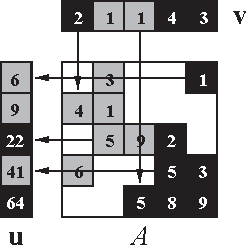
\includegraphics{img/communication}
	\caption{Communication involved following Algorithm \ref{alg:matvec} for a matrix distributed as in Figure \ref{fig:partition}. Vertical arrows represent step (0) while horizontal ones represent step (2).}
	\label{fig:communication}
\end{figure}



As our main interest is to \textbf{minimize} the time spent by the parallel machine computing this sparse matrix-vector multiplication, we need to compute explicitly the cost of Algorithm \ref{alg:matvec}: we can immediately note that such algorithm, which follows the Bulk Synchronous Parallel model\cite{bsp_paper}, consists of two communication supersteps separated by a computation superstep.

The time spent by a parallel machine in a computation superstep is exactly the time taken by the processor that finishes last: more formally, the time cost of step (1):

\begin{align}
	T_{(1)} = \max_{0 \leq s < p } |A_s|.
	\label{eq:T_comp}
\end{align}

It is easy to understand that, in order to have efficient parallelization, the computation load has to be distributed evenly. Usually, however, it is not possible to achieve a perfect load balance (e.g. when dividing up an odd number of computations among an even number of processors) and we have to reason in term of allowed imbalance $\varepsilon$. Consequently, we impose the following hard constraint about the maximum size of the subsets of nonzeros assigned to each processor, according to \cite[eq.~4.27]{BSP}:

\begin{align}
\max_{0 \leq s <p} |A_s| \leq (1+\varepsilon) \frac{N}{p}.
	\label{eq:balance}
\end{align}

Typical values for the allowed $\varepsilon$ in this constraint are 0.03, i.e. a 3\% imbalance.

It is reasonable, after all, that the problem of finding an efficient way of performing this computation step boils simply down to a hard constraint for the data distribution. This is because, after all, we still have to perform all the multiplications of the form $a_{ij} v_j$, no matter our choice. 

The communication costs, represented by the first and last supersteps in Algorithm \ref{alg:matvec}, are the most interesting aspect about maximizing the efficiency of a parallel sparse-matrix vector multiplication algorithm, as there is extreme variability. As a simple example, suppose $p=2$: the difference between a ``checkered'' distribution (i.e. the nonzeros are assigned alternatingly to the processors, looking at both the rows and the columns) and a distribution in which every nonzero is assigned to processor 0 (forgetting for one moment about the load balance), is very large. In the first case we have the maximum possible communication, regardless of the vector distribution, whereas in the second case there is no communication at all.

Previously, we claimed that the matrix and both the vectors have to be partitioned: in reality it is sufficient to consider only the problem of distributing the nonzeroes, and the partitioning of the vector can be executed according to this: because of the structure of the communication supersteps in Algorithm \ref{alg:matvec}, we have that communication is required if and only if the rows/columns of the matrices are \emph{cut}, i.e. assigned to more than one processor.

If a full column of our matrix $A$ is assigned to the same processor, we can freely assign the first component of $v$ to the same processor, eliminating completely one source of communication (namely, the fan-out for that column). The same reasoning can be extended for the rows. This simplification is possible because imposing a hard constraint similar to \eqref{eq:balance} also to the vector distribution is not very helpful, as it only affects the time of linear vector operations outside the matrix-vector multiplication, which are in generally much cheaper \cite[Sec.~3]{mondriaan}. 

We can describe more formally the communications cost, following the notation of \cite[Def.~2.1]{mondriaan}: let $A_0,\dots,A_{p-1}$ be a $p$-way (with $p \geq 1$) partitioning of the sparse matrix $A$ of size $m \times n$. Let $\lambda_i$ denote the number of processors which have a nonzero of row $i$ and let $\mu_j$ be the number of processors that have a nonzero of column $j$.

Then the total time costs for the communication steps in our Algorithm \ref{alg:matvec} are:

\begin{align}
	\begin{aligned}
	T_{(0)} &= \sum_{j=0}^{n-1} (\mu_j -1), \\
	T_{(2)} &= \sum_{i=0}^{m-1} (\lambda_i -1).
\end{aligned} \label{eq:T_comm}
\end{align}

These costs are quite straightforward: it is reasonable to assume that the owner of the appropriate vector component is between the ones that have a nonzero in that row/column, and therefore one communication is not necessary.

Adding up these costs together, we define the \textbf{communication volume} $V$ of the considered partitioning as

\begin{align}
	V := V(A_0,\dots,A_{p-1}) = T_{(0)} + T_{(2)} = \sum_{i=0}^{m-1} (\lambda_i -1) + \sum_{j=0}^{n-1} (\mu_j-1).
	\label{eq:volume}
\end{align}

As we can see, the communication volume $V$ depends entirely on the matrix $A$ and the considered partitioning. Therefore, the problem of minimizing the cost of a matrix-vector multiplication is shifted toward finding an efficient way of distributing the sparse matrix among the available processors, such that our balance constraint \eqref{eq:balance} is satisfied. The following sections and chapters and, ultimately, this whole Master Thesis, are therefore dedicated to it.

\section{Hypergraph model}

The problem of distributing the nonzero of a matrix in order to minimize the communication volume, or, in short, the matrix partitioning problem, can also be viewed from the graph theory point of view. We recall that a (unweighted, undirected) graph $G=(V,E)$ is a set of vertices (or nodes) $V$ and edges $E$ which connect them. 

The graph partitioning problem has always been used to model the load balancing in parallel computing \cite{parallel_hypergraph}: data are represented as vertices, while their connections (the dependencies) are represented with edges. 

For a more rigorous definition of the graph partitioning problem, we follow the notation given in \cite{hypergraph_model},  performing the simplification in which all the edges have unitary weight. Given the graph $G=(V,E)$ we say that $(V_0,\dots,V_{p-1})$ is a $p$-way partitioning of $G$ if all these subsets are nonempty, mutually disjoint and their union is the whole set of nodes $V$. 

Moreover, we can consider a balance criterion similar to \eqref{eq:balance}:
\begin{align}
	\max_{0\leq s <p}	|V_s| \leq (1+\varepsilon)\frac{|V|}{p},
	\label{eq:balance_hypergraph}
\end{align}

where $\varepsilon$, similarly as before, represents the allowed imbalance.

Now, given a partition $(V_0,\dots,V_{p-1})$ of the graph $G$, we say that the edge $e=(i,j)$ is \emph{cut} if $i \in V_k, j \in V_l$, with $k \neq l$; otherwise, it is said to be \emph{uncut}. Previously, we claimed that communication during the parallel matrix-vector multiplication can be avoided if a row/column is uncut, and here the goal is the same: we want to minimize the \emph{cutsize}, i.e. the number of edges cut.

However, despite all the similarities between the matrix partitioning problem and the graph partitioning one, it has been shown \cite{hypergraph_model}\cite{zoltan_worth-it},  that this cut-edge metric is not an accurate representation of the communication volume. Additional criticism \cite{hendrickson_emperor} comes from the fact that the graph partitioning approach can only handle square symmetric matrices. It was also shown \cite{hendrickson_kolda} that these disadvantages hold for all application of graph partitioning in parallel computing, and not only our problem of matrix partitioning for sparse matrix-vector multiplication. 

In \cite{hypergraph_model} it is shown that a more correct way of modeling the matrix partitioning problem is through the concept of hypergraph partitioning.

A hypergraph is simply a generalization of a graph: we do not consider edges that connect two nodes, but rather \emph{hyperedges}, which are subsets of nodes. Apart from considering only non-empty hyperedges, note that there is no other restriction on a cardinality of a hyperedge.

Hypergraphs, and in particular the hypergraph partitioning problem are already well known in literature: they have a natural application in the designing of integrated circuits (VLSI), in finding efficient storage of large databases on disks, and data mining \cite{vlsi}, as well as urban transportation design and study of propositional logic \cite{papa_hypergraph}.

Because of this extensive literature, translating our matrix partitioning problem to a hypergraph partitioning problem seems quite convenient, as all the methods already developed can be analyzed and employed also in our case.

Figure \ref{fig:hypergraph} shows an example of such hypergraph. Each colored set represents a different hyperedge; we can see that we can have hyperedges which contain only one node.

\begin{figure}[h]
	\centering
	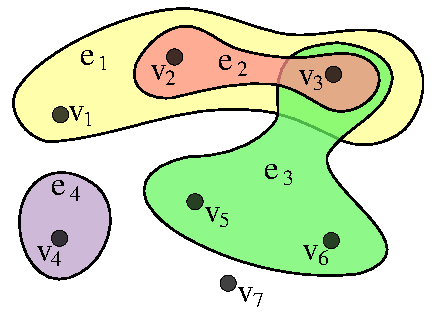
\includegraphics{img/hypergraph}
	\caption{Hypergraph example. Image courtesy of Wikimedia Commons: \url{https://commons.wikimedia.org/wiki/File:Hypergraph-wikipedia.svg}.}
	\label{fig:hypergraph}
\end{figure}

The definition of hypergraph partitioning problems is identical to the case of simple graph, with the difference that now we don't have cut edges, but cut hyperedges: given the hyperedge $e=\{e_1,\dots,e_k\}$, we say that $e$ is cut if there are $i,j$ such that $e_i \in V_r, e_j \in V_s$, with $r \neq s$, i.e. at least two nodes belong to different sets of the partition. As usually, we want to minimize the cut hyperedges.

If, similarly to \eqref{fig:communication}, we define $\lambda_e$ as the number of different sets the vertices in the hyperedge $e$ are assigned to, we have that the total cost of the partition $(V_0,\dots,V_p)$ is:
\begin{align}
	C = C(V_0,\dots,V_{p-1}) = \sum_{e \in E} (\lambda_e -1).
	\label{eq:cost_hypergraph}
\end{align}

We can see how closely these equations resemble the ones given in the previous section: it is clear that the hypergraph partitioning problem closely resembles our original matrix partitioning problem.

Note that the partitioning hypergraph model, along with the simple graph partitioning problem, are known to be NP-hard \cite[Ch.~6]{lengauer}. 

Now, we will describe three possible models for the decomposition of a sparse matrix into a hypergraph, and discuss their advantages and disadvantages.

In the \textbf{column-net} model, our matrix $A$ is represented as a hypergraph for a row-wise decomposition: rows of the matrix are nodes ($V=\{v_1,\dots,v_m\}$, while columns are hyperedges ($E= \{e_1,\dots,e_n\}$). We have that the node $v_i$ belongs to the hyperedge $e_j$ (in short $v_i \in e_j$) if and only if $a_{ij} \neq 0$. With this model, we have that the size of the hyperedge $e_j$ is exactly the number of nonzeros in that column, whereas the node $v_i$ belongs exactly to as many hyperedges as there are nonzeros in that row.

As already said, performing a partitioning on the hypergraph consists in assigning each vertex to one of the sets $V_0,\dots,V_{p-1}$. In this model, this corresponds to assigning a row completely to a processor.

However, as vertices are not exactly nonzeros of our matrix, \eqref{eq:balance} and \eqref{eq:balance_hypergraph} are not exactly equivalent; we need to adjust our balance constraint by introducing a weight for each vertex, as in \cite[Def.~4.34]{BSP}. For $v_j \in V$, we define its weight $c_j$ as

\[
	c_j := |\{\;i : \;a_{ij} \neq 0\}|,
\]

which simply is the number of nonzeros in row $i$ of the matrix $A$. Note that, following the same notation as in the previous section, we can see the total number of nonzeros $N$ as $N = \sum_{v_j \in V} c_j$.

Our modified balance constraint is as follows:

\begin{align}
	\max_{0 \leq s <p}	W(V_s) := \max_{0 \leq s <p} \sum_{v_j \in V_s} c_j \leq (1 + \varepsilon) \frac{N}{p}.
	\label{eq:balance_columnet}
\end{align}

The \textbf{row-net} model is very similar the one just described (as can be guessed from the name): it is exactly the symmetrical of the colum-net model, in the sense that now rows are hyperedges and columns are vertices of the hypergraph. The reasoning just described applies also to this model, with the little modification that now the weight of a vertex is the number of nonzeros in that column.

We see how the column-net model and row-net model have the advantage of fully assigning a row (or a column) to a processor; this has the advantage of eliminating completely one source of communication in our parallel sparse matrix-vector multiplication algorithm (respectively, the fan-in and fan-out). However, this advantage can easily become a weakness, because now the partitioning is forcedly 1-dimensional, and this is usually a too-strong restriction.

Now, as last example of possible decomposition of a matrix into a hypergraph, and as a partial address to the drawbacks of the previous two models, we will describe a 2-dimensional approach, the so-called \emph{fine-grain} model \cite{hypergraph_finegrain}.

In this model, we have that the $N$ nonzeros are the vertices ($V = \{ v_1,\dots,v_N\}$) and the $m$ rows and $n$ columns are hyperedges ($E = E_r \cup E_c = \{ e_1,\dots,e_m \} \cup \{e_{m+1},\dots,e_{m+n}\}$). With this notation, $E_r$ represents the row hyperedges and $E_c$ represents the column hyperedges.

The relationship between the vertices and the hyperedges is fairly obvious: $v_k = a_{ij}$ is in both $e_i$ and $e_{m+j}$.

Now, as the vertices correspond exactly to nonzeros of our matrix, we can use the original equation \eqref{eq:balance_hypergraph} as balance constraint; if we combine this to \eqref{eq:cost_hypergraph}, which describes the cost of a hypergraph partition, we can clearly see how this is identical to our original matrix partitioning problem, described by \eqref{eq:balance} and \eqref{eq:volume}.

On a higher level, one of the benefits of this decomposition model is easy to understand: we have a lot of freedom and we can assign individually each nonzero to a different partition. Similarly as before, however, this advantage can easily become a drawback because now the size of the hypergraph is consistently larger, with $N$ vertices compared to $m$ and $n$ of the previous two models. Thus, computations on the fine-grain model take substantially more time than row-net or column-net models and therefore there is a restriction on the size of the problem that can be efficiently solved.

\section{Earlier work}

As hypergraph partitioning has a wide variety of applications, it has been extensively studied in literature.

In the previous section, we already mentioned the row-net and column-net models \cite{hypergraph_model}, and a more fine-grained approach, \cite{hypergraph_finegrain}. In \cite{hypergraph_revisiting} Uçar and Aykanat first employ an elementary 1-dimensional hypergraph model, and then transform it in several ways to hypergraph models suitable for symmetric and unsymmetric partitionings; these models include also the input and output vectors, and therefore a few extra vertices are added.

A different 2-dimensional approach is given by the \emph{coarse-grain} method \cite{hypergraph_coarsegrain}, in two phases: first it applies the column-net hypergraph model and obtains a row partitioning of the matrix in $p$ parts, then it performs  a multi-constraint column partitioning in $q$ parts, yielding a final 2-D cartesian partitioning in $p \times q$ parts. 

Alternatively, Vastenhouw and Bisseling proposed a 2-dimensional recursive method for data distribution \cite{mondriaan}. 

An interesting model recently proposed by Pelt and Bisseling \cite{mediumgrain}, called \textbf{medium-grain}, is a further exploitation of 2-dimensional partioning, and it has produced good results. As this model is at the base of our work, a more detailed explanation will be given in Section \ref{sec:mediumgrain}.

Also, the matrix structure has to be taken into account to devise specifically targeted methods: while initially devised for structurally symmetric matrices \cite{hypergraph_model}, the hypergraph-based approach was shown to be efficient also in case of rectangular matrices, by Pinar et al.\cite{pinar1996}, for the partitioning of rectangular Linear Programming matrices.

Hu, Maguire and Blake present in \cite{hu2000} an algorithm for nonsymmetric matrices that performs row and column permutations, getting a bordered block diagonal form and then trying to assign matrix rows such that the number of cut columns is minimized.

In general, as there is such a wide variety of different methods and model, it might be difficult to choose the best one, given a matrix to partition. {\c{C}}ataly{\"u}rek, Aykanat, and U{\c{c}}ar propose a partitioning recipe \cite{catalyurek_recipe} that chooses a partitioning method according to some matrix characteristics.

There also available a modest number of software partitioners that implements some of the methods and models just discussed, along with other: among the sequential ones we have PaToH (a multilevel Partitioning Tool for Hypergraphs) \cite{patoh}, hMetis \cite{hmetis} (specifically tageted at partitioning hypergraphs for VLSI design), Mondriaan \cite{mondriaan} (more specifically designed to solve the matrix partitioning problem), MONET (Matrix Ordering for minimal NET-cut)\cite{hu2000}, while among the parallel ones we have Zoltan-PHG (Parallel Hypergraph Partitioner) \cite{parallel_hypergraph}.

All of these partitioners produce very different results, with respect to both solution quality and execution time, despite having at the core the same method for finding good initial solutions, namely the Kernighan-Lin method \cite{kernighan_lin}, with the optimizations of Fiduccia-Mattheyses \cite{fiduccia}. This method (often handily abbreviated with KLFM from the initials of the authors involved), originally designed for bipartitioning graphs, is a local search heuristic: given a partitioning that obeys the balance constraint \eqref{eq:balance}, applies a series of small changes to find improvement in the quality solution.

To solve large instances, all these partitioners use a multi-level method: the large problem is progressively coarsened until a smaller instance is obtained, then the problem is solved on this small instance and the solution is gradually uncoarsened, with a refinement at each step to improve the solution quality.

Finally, these existing software partitioners are all based on \emph{recursive bisection}: instead of partitioning the hypergraph directly into the desired number of parts, they operate a sequence of bisection of the partitions. This is a good semplification in the sense that efforts on finding methods for good bipartitioning can be re-employed, and also because splitting a hypergraph in just two parts is much easier; but there is also a major flaw that, using this recursive bisection, we might not be able to reach the same quality of a solution with direct splitting into the desired number of parts.

\section{Medium-grain model} \label{sec:mediumgrain}

All of the possible ways of translating the matrix partitioning problem into the hypergraph partitioning one have different advantages and drawbacks: the 1-dimensional ones, row-net and colum-net, eliminate completely one source of communication but are somewhat too restricting; fine-grain, on the contrary, does not provide any kind of restriction on the partitioning, but resulting in too large to manage hypergraph.

We will now describe a model proposed by Pelt and Bisseling \cite{mediumgrain} which can be described as a sort of middle ground between these two kinds of models: the resulting partitioning is 2-dimensional by design (thus avoiding the restriction of the row-net and column-net), but it still imposes clusters of nonzeros from the same rows and columns to be assigned to same processor, thus avoiding the main disadvantage of the fine-grain.

The key of this model lies in splitting our original matrix $A$ in two parts, $A_r$ and $A_c$, i.e. we have that $A_r + A_c = A$; then we proceed to construct the auxiliary block-matrix $B$, of size $(m+n) \times (m+n)$, as:

\begin{align}
	B:=	\begin{bmatrix}
		I_n & A_r^T \\
		A_c & I_m
	\end{bmatrix},
	\label{eq:Bmatrix}
\end{align}

where $I_n$ and $I_m$ denote, respectively, the identity matrices of size $n$ and $m$. Then the final hypergraph is obtained by applying the row-net model to this matrix $B$. 

Figure \ref{fig:mediumgrain-1} illustrates this process for a $3 \times 6$ rectangular matrix $A$.

\begin{figure}[h]
	\centering
	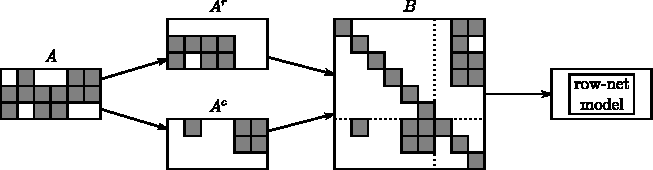
\includegraphics{img/mg-1}
	\caption{Construction of the hypergraph according to the medium-grain model.}
	\label{fig:mediumgrain-1}
\end{figure}

After we apply the row-net model and obtain a partitioning of the hypergraph, we only consider the parts of $B$ which corresponded to $A_r$ and $A_c$ and we assemble back the original matrix $A$, with a new partitioning.

Figure \ref{fig:mediumgrain-2} illustrates this process of translating the hypergraph partitioning into a partitioning of our original matrix $A$.

\begin{figure}[h]
	\centering
	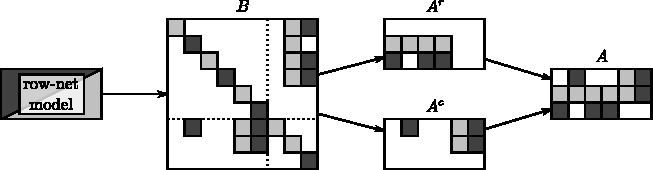
\includegraphics{img/mg-2}
	\caption{Process of obtaining a matrix partitioning starting from a partitioning of the hypergraph following the medium-grain model. In this case $p=2$.}
	\label{fig:mediumgrain-2}
\end{figure}

Because we are partitioning the matrix $B$ with the row-net models, we can understand the meaning of $A_c$ and $A_r$. The first is left as-is, while the second is transposed; then, when partitioning 1-dimensionally such that the columns are kept together, we see that elements within the same column of $A_c$ are kept together, while elements in the same row of $A_r$ (a column of $A_r^T$) are kept together. The resulting partitioning is then fully 2-dimensional because we have clusters of nonzeros: rows for $A_r$ and columns for $A_c$ (hence the subscripts).

The diagonal elements of $B$ are used only to compute the communication volume: to understand this, consider the $k$-column of $A$. The corresponding nonzeros can be found in the part related to $A_c$ (i.e. $b_{n+j,k}$, for $1 \leq j \leq m$) and related to $A_r^T$ (i.e. $b_{k,n+j}$, $1 \leq j \leq m$). If both these parts are nonempty, i.e. the $k$-th column of $A$ was not fully assigned to either $A_r$ or $A_c$, we need to be careful when partitioning, because if they get assigned to different processors we have indeed communication in Algorithm \ref{alg:matvec}.

Therefore the diagonal nonzero $B_{k,k}$, which is assigned to the same processor as the part belonging to $A_c$, but it placed in the same row as the part belonging to $A_r$, serves exactly the purpose of keeping track of the partitioning, such that the computation of the communication volume is correct \cite[Th.~3.1]{mediumgrain}. Note that implementation-wise there is no need to have the complete diagonal of $B$: we put a nonzero if and only if the corresponding row of $A_r^T$ and column of $A_c$ are nonempty.

Experimental results, performed with both the Mondriaan software partitioner \cite{mondriaan} and PaToH \cite{patoh} seemed to confirm that this model has indeed some advantages to column-net, row-net and fine-grain, both for partitioning time and solution quality.

Because of these good results, it is interesting to investigate further the properties of this model, in two possible directions.

First of all, as the outcome of the medium-grain model depends consistently on the intial split of $A$ into $A_r$ and $A_c$, therefore it is interesting to investigate the quality of the algorithm originally proposed in \cite{mondriaan}; secondly, we will try to develop a fully iterative method that employs the medium-grain model, where a full multi-level partitioning is performed at each iteration and computational time is traded for solution quality.
